%% Introduction
\section*{Introduction}

\lettrine[lines=2]{A}{ctive} Noise Control 
(ANC) is a method used in a wide variety of applications. Research in creating silent zones is being conducted \cite{SilentZones}, improving room acoustics using multiple loudspeakers \cite{CAPS} and is already available in various headphones.
\\\\
Noise canceling headphones are used in various environments with different noise characteristics. These characteristics vary from periodic low frequency noise (10 Hz -- 200 Hz), e.g. from machinery and helicopter rotors \cite{LowFrequency}, to mid-range frequency noise (200 Hz -- 4000 Hz), e.g. speech \cite{MidFrequency}, to high frequency noise (4 $k$Hz -- 20 $k$Hz), e.g. turbine noise \cite{LowFrequency}. The high frequency noise is passively attenuated by using a closed headphone cup \cite{naturalAttenuation}, and present consumer headphones are able to attenuate low frequency periodic noise \cite{naturalAttenuation}. The attenuation of speech using ANC in present market ANC headphones is shown in figure \ref{fig:ANCcompare}. \\\\

%\footnote{Numbers and sources will be added to the statements}.   
%%ANC are used by companies such as Bang \& Olufsen and Lyngdorf Audio in their proprietary technology as Active Room Compensation\texttrademark and RoomPerfect\texttrademark respectively, to control noise in a room using loudspeakers. Headphone industries have adapted it into cancellation of noise and is used 

This paper focuses on improving attenuation of speech. Hence speech will be seen as the only noise source. The solution proposed is based on a digital feedforward system using Filtered-$x$ Least Mean Squares (FXLMS). The solution is chosen due to it being the optimal system for non-stationary signals \cite{Hansen2}. The general solutions in ANC are described thoroughly by Hansen et al. \cite{Hansen}.

\begin{figure}[H]
	\centering
	\tikzsetnextfilename{ComparedConusmerHP}
	% This file was created by matlab2tikz.
%
%The latest updates can be retrieved from
%  http://www.mathworks.com/matlabcentral/fileexchange/22022-matlab2tikz-matlab2tikz
%where you can also make suggestions and rate matlab2tikz.
%
\definecolor{mycolor1}{rgb}{0.00000,0.44700,0.74100}%
\definecolor{mycolor2}{rgb}{0.85000,0.32500,0.09800}%
\definecolor{mycolor3}{rgb}{0.92900,0.69400,0.12500}%
\definecolor{mycolor4}{rgb}{0.49400,0.18400,0.55600}%
%
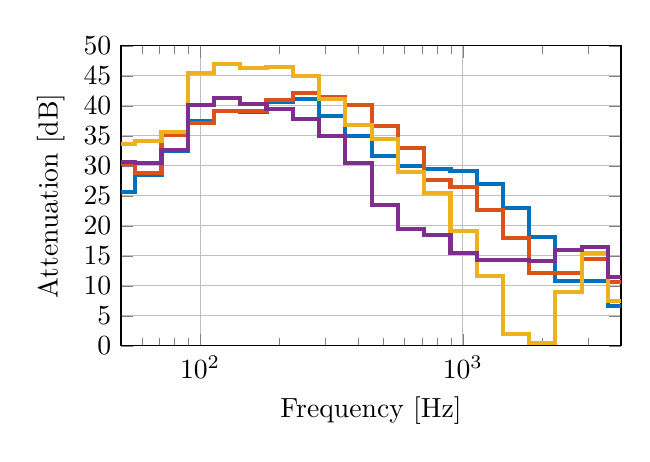
\begin{tikzpicture}

\begin{axis}[%
width=2.5in,
height=1.5in,
at={(1.011in,0.642in)},
scale only axis,
xmode=log,
xmin=50,
xmax=4000,
xlabel={Frequency [Hz]},
xmajorgrids,
%xmajorgrids,
%ymajorgrids,
%xminorgrids,
ymin=0,
ymax=50,
ytick={0,5,...,50},
ylabel={Attenuation [dB]},
ymajorgrids,
axis background/.style={fill=white},
title style={font=\bfseries},
%title={Comparison of Smoothened curves},
legend style={legend cell align=left,align=left,draw=white!15!black}
]
%\addplot[const plot,color=mycolor1,solid,forget plot,thick] plot table[row sep=crcr] {%
%	28.4	15.7\\
%	35.7	15.1\\
%	45	12.4\\
%	56.6	14\\
%	71.3	16.3\\
%	89.7	18.8\\
%	113	19.6\\
%	142	19.5\\
%	179	20.3\\
%	225	20.4\\
%	284	19.2\\
%	357	17.4\\
%	450	15.7\\
%	566	15.1\\
%	713	14.7\\
%	897	14.5\\
%	1.13e+03	13.5\\
%	1.42e+03	11.5\\
%	1.79e+03	9.08\\
%	2.25e+03	5.31\\
%	2.84e+03	5.51\\
%	3.57e+03	3.03\\
%	4.5e+03	2.37\\
%	5.66e+03	2.81\\
%	7.13e+03	3.07\\
%	8.97e+03	3.24\\
%	1.13e+04	1.16\\
%	1.42e+04	0.032\\
%	1.79e+04	0.598\\
%	2e+04	-0.763\\
%};
%\addplot[const plot,color=mycolor2,solid,forget plot,thick] plot table[row sep=crcr] {%
%	28.4	14.7\\
%	35.7	15.3\\
%	45	15.2\\
%	56.6	14.2\\
%	71.3	17.6\\
%	89.7	18.7\\
%	113	19.5\\
%	142	19.5\\
%	179	20.4\\
%	225	21.3\\
%	284	20.8\\
%	357	19.8\\
%	450	18.4\\
%	566	16.5\\
%	713	13.4\\
%	897	13.2\\
%	1.13e+03	11.4\\
%	1.42e+03	8.6\\
%	1.79e+03	6.11\\
%	2.25e+03	6.07\\
%	2.84e+03	7.27\\
%	3.57e+03	4.99\\
%	4.5e+03	2.6\\
%	5.66e+03	2.91\\
%	7.13e+03	1.03\\
%	8.97e+03	2.02\\
%	1.13e+04	-0.338\\
%	1.42e+04	-0.849\\
%	1.79e+04	-0.618\\
%	2e+04	-2.19\\
%};
%\addplot[const plot,color=mycolor3,solid,forget plot,thick] plot table[row sep=crcr] {%
%	28.4	18.1\\
%	35.7	19\\
%	45	17.1\\
%	56.6	16.5\\
%	71.3	18.6\\
%	89.7	22.8\\
%	113	23.6\\
%	142	23.3\\
%	179	23.5\\
%	225	22.6\\
%	284	20.4\\
%	357	18.4\\
%	450	17.2\\
%	566	14.5\\
%	713	12.7\\
%	897	9.48\\
%	1.13e+03	5.89\\
%	1.42e+03	1.04\\
%	1.79e+03	0.132\\
%	2.25e+03	4.45\\
%	2.84e+03	7.76\\
%	3.57e+03	3.73\\
%	4.5e+03	2.58\\
%	5.66e+03	2.46\\
%	7.13e+03	1.18\\
%	8.97e+03	1.16\\
%	1.13e+04	0.0281\\
%	1.42e+04	-0.34\\
%	1.79e+04	-0.623\\
%	2e+04	-1.08\\
%};
%\addplot[const plot,color=mycolor4,solid,forget plot,thick] plot table[row sep=crcr] {%
%	28.4	18.6\\
%	35.7	16.5\\
%	45	15.5\\
%	56.6	15.5\\
%	71.3	16.6\\
%	89.7	20.3\\
%	113	20.4\\
%	142	20\\
%	179	19.6\\
%	225	18.9\\
%	284	17.4\\
%	357	15.3\\
%	450	11.8\\
%	566	9.77\\
%	713	8.89\\
%	897	7.71\\
%	1.13e+03	6.86\\
%	1.42e+03	7.05\\
%	1.79e+03	7.37\\
%	2.25e+03	7.85\\
%	2.84e+03	8.24\\
%	3.57e+03	5.7\\
%	4.5e+03	3.78\\
%	5.66e+03	3.02\\
%	7.13e+03	1.43\\
%	8.97e+03	1.33\\
%	1.13e+04	1.58\\
%	1.42e+04	0.0462\\
%	1.79e+04	-1.02\\
%	2e+04	-0.621\\
%};
%\end{axis}

%% 20 log
\addplot[const plot,color=mycolor1,solid,line width=1.5pt,forget plot] plot table[row sep=crcr] {%
	28.4	30.6\\
	35.7	31.3\\
	45	25.7\\
	56.6	28.5\\
	71.3	32.4\\
	89.7	37.4\\
	113	39.1\\
	142	39\\
	179	40.6\\
	225	41.2\\
	284	38.3\\
	357	35\\
	450	31.7\\
	566	30\\
	713	29.4\\
	897	29.1\\
	1.13e+03	27\\
	1.42e+03	23\\
	1.79e+03	18.2\\
	2.25e+03	10.8\\
	2.84e+03	10.8\\
	3.57e+03	6.62\\
	4.5e+03	4.92\\
	5.66e+03	5.21\\
	7.13e+03	5.95\\
	8.97e+03	5.98\\
	1.13e+04	2.27\\
	1.42e+04	-1\\
	1.79e+04	0.842\\
	2e+04	-1.38\\
};
\addplot[const plot,color=mycolor2,solid,line width=1.5pt,forget plot] plot table[row sep=crcr] {%
	28.4	29.3\\
	35.7	30.1\\
	45	30.3\\
	56.6	28.8\\
	71.3	35.2\\
	89.7	37.2\\
	113	39.1\\
	142	39.2\\
	179	41\\
	225	42.2\\
	284	41.5\\
	357	40.1\\
	450	36.7\\
	566	33\\
	713	27.7\\
	897	26.5\\
	1.13e+03	22.7\\
	1.42e+03	17.9\\
	1.79e+03	12.1\\
	2.25e+03	12.1\\
	2.84e+03	14.4\\
	3.57e+03	10.6\\
	4.5e+03	5.72\\
	5.66e+03	5.17\\
	7.13e+03	2.13\\
	8.97e+03	4.17\\
	1.13e+04	-0.138\\
	1.42e+04	-0.907\\
	1.79e+04	-1.96\\
	2e+04	-4.33\\
};
\addplot[const plot,color=mycolor3,solid,line width=1.5pt,forget plot] plot table[row sep=crcr] {%
	28.4	36.2\\
	35.7	38.5\\
	45	33.6\\
	56.6	34.2\\
	71.3	35.6\\
	89.7	45.5\\
	113	46.9\\
	142	46.3\\
	179	46.5\\
	225	44.9\\
	284	41.1\\
	357	36.8\\
	450	34.5\\
	566	29\\
	713	25.5\\
	897	19.1\\
	1.13e+03	11.6\\
	1.42e+03	1.91\\
	1.79e+03	0.429\\
	2.25e+03	9.03\\
	2.84e+03	15.5\\
	3.57e+03	7.47\\
	4.5e+03	4.95\\
	5.66e+03	4.31\\
	7.13e+03	2.18\\
	8.97e+03	2.87\\
	1.13e+04	0.264\\
	1.42e+04	-0.554\\
	1.79e+04	-2.08\\
	2e+04	-2.36\\
};
\addplot[const plot,color=mycolor4,solid,line width=1.5pt,forget plot] plot table[row sep=crcr] {%
	28.4	37.2\\
	35.7	33.9\\
	45	30.7\\
	56.6	30.4\\
	71.3	32.7\\
	89.7	40.2\\
	113	41.3\\
	142	40.3\\
	179	39.5\\
	225	37.8\\
	284	34.9\\
	357	30.5\\
	450	23.4\\
	566	19.5\\
	713	18.4\\
	897	15.4\\
	1.13e+03	14.3\\
	1.42e+03	14.3\\
	1.79e+03	14.1\\
	2.25e+03	16\\
	2.84e+03	16.4\\
	3.57e+03	11.5\\
	4.5e+03	7.26\\
	5.66e+03	6.34\\
	7.13e+03	2.99\\
	8.97e+03	2.87\\
	1.13e+04	2.9\\
	1.42e+04	0.784\\
	1.79e+04	-1.51\\
	2e+04	-1.74\\
};
\end{axis}
\end{tikzpicture}%
	\caption{Denon AH-GC20, Bose QC25, Bose QC15 and B\&O H8 measured in anechoic chamber, averaged over five measurements where the headphones was refitted between measurements. Results are filtered using a class 0 1/3 octave filter bank \cite{OctaveBand}.}
	\label{fig:ANCcompare}
\end{figure}



The problem of a feedforward system is the dependency of the system delay being smaller than the propagation time from the noise measured (1), to the error microphone (3), shown in \autoref{fig:SystemOverview}.
\begin{figure}[H]
	\centering
	%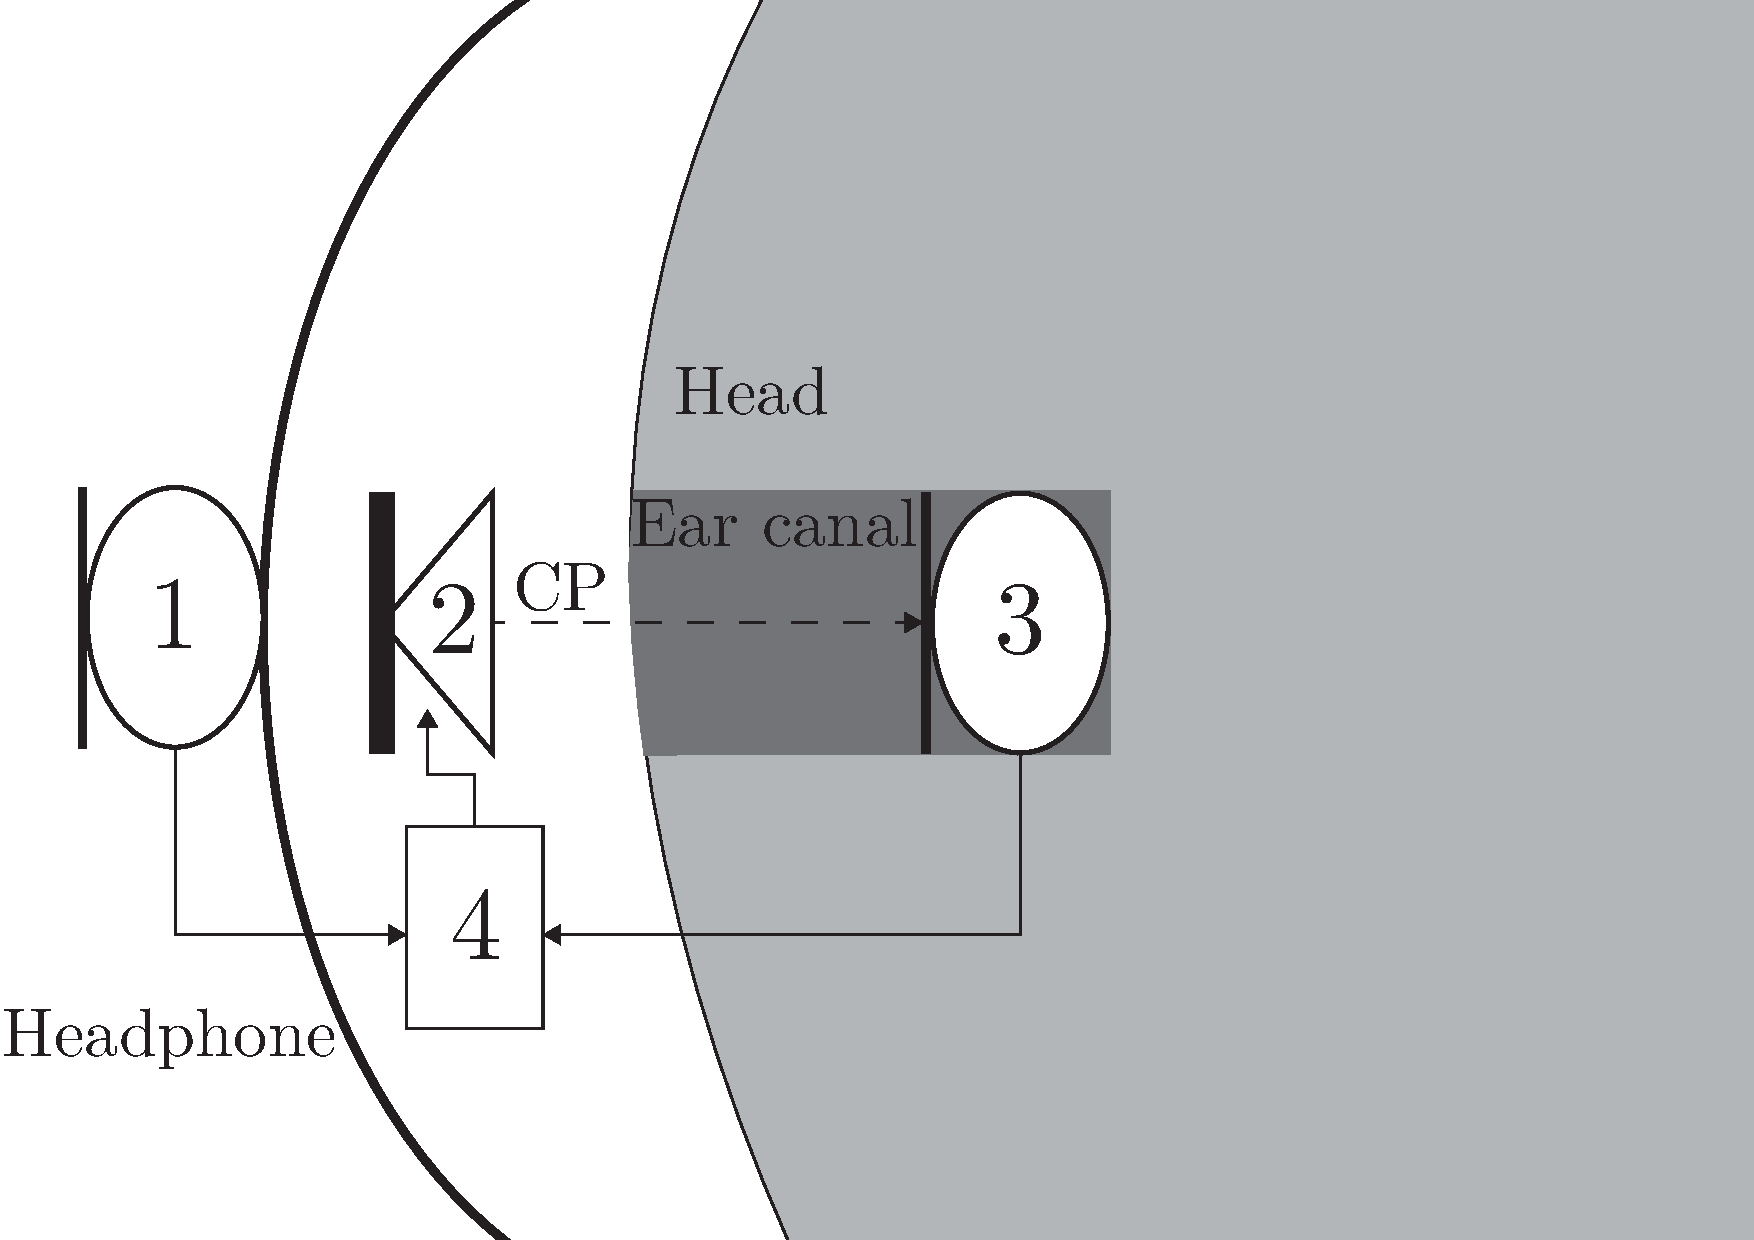
\includegraphics[width=1\columnwidth]{figures/ArticleIllustrations/BasicOverviewZoomed}
	\tikzsetnextfilename{BasicOverviewZoomed}
	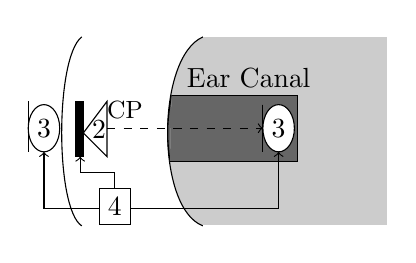
\begin{tikzpicture}
\draw [](-2.22,2.52) node (v1) {} .. controls (-2.56,2.26) and (-2.56,0.34) .. (-2.22,0.12) node (v2) {};

\draw [draw=black,fill=black!20](-0.68,2.52) node (v1) {} .. controls (-1.28,2.26) and (-1.28,0.34) .. (-0.68,0.12) node (v2) {};
\draw [white, fill=black!20](-0.68,2.52) -- (1.66,2.52) -- (1.66,0.12) -- (-0.68,0.12);


\draw [draw=black,fill=black!60](-1.08,1.78) node (v1) {} .. controls (-1.14,1.44) and (-1.14,1.24) .. (-1.1,0.94) node (v2) {};
\draw [draw=black,fill=black!60](-1.08,1.78) -- (0.52,1.78) -- (0.52,0.94) -- (-1.1,0.94);


\draw [draw=black,fill=white] (0.28,1.36) node (v3) {3} ellipse (0.2 and 0.3);
\draw [draw=black,fill=black](0.08,1.66) -- (0.08,1.06);

\draw [draw=black,fill=white] (-2.7,1.36) node (v3) {3} ellipse (0.2 and 0.3);
\draw [draw=black,fill=black](-2.9,1.7) -- (-2.9,1.06);


\draw [draw=black,fill=black] (-2.2,1.7) rectangle (-2.3,1);
\draw (-2.2,1.3) -- (-1.9,1.7) -- (-1.9,1) -- (-2.2,1.3);
\node at (-2,1.34) {2};


\draw[->,dashed] (-1.9,1.36) node[right=6.5,above]{\small{CP}}-- (0.08,1.36);
\draw  (-1.6,0.6) rectangle node{4}(-2,0.14);
\draw [->](-2,0.34) -- (-2.7,0.34) -- (-2.7,1.06);
\draw [->](-1.6,0.34) -- (0.28,0.34) -- (0.28,1.06);
\draw [->](-1.8,0.6) -- (-1.8,0.8) -- (-2.24,0.8) -- (-2.24,1);
\node at (-0.1,2) {Ear Canal};
\end{tikzpicture}
	\caption{Simplified circumaural ANC Headphone fitted on an ear. Showing the reference microphone (1), a headphone loudspeaker (2), an error microphone (3) and a DSP (4).}
	\label{fig:SystemOverview}
\end{figure}
In a real-time system, delays are introduced by sampling and processing a signal. For instance, using a cost-wise $\Sigma\Delta$-converter a sampling/conversion delay is introduced. The specific delay values for a TLV320AIC3204 can be seen in \autoref{tab:DelayResults}.

%delay in the range of 220 $\mu$s to 880 $\mu$s is introduced, depending on a sampling frequency of 192 kHz to 48 kHz respectively.



\begin{table}[H]
	\centering
	\begin{tabular}{|l|l|l|l|}
	\hline
	$f_s$ {[}$k$Hz{]} & 48 & 96 & 192 \\ \hline
	Delay {[}$\mu$s{]} & 900 & 450 & 225 \\ \hline
	Delay {[}samples{]} & 43 & 43 & 43 \\ \hline
\end{tabular}
	\caption{The measured delay of TLV320AIC3204 in both time and samples at different sampling frequencies.}
	\label{tab:DelayResults}
\end{table}

Assuming a $\text{0}^{\circ}$ angle of incident, which is the ideal case, the reference microphone must be placed 75.5 $m$m -- 302 $m$m further out from the error microphone, to compensate for the delay. Instead a Linear Prediction (LP) scheme is proposed as a solution. In speech encoding Wiener filtering is often used \cite{Speech} therefore Wiener filtering is the choosen prediction method.
% This reduces computation time and overall
%Consumer ANC headphones has a bandwidth that does not cover the entire frequency area of speech. This paper examines how to extend the bandwidth.
%To increase bandwidth a prediction algorithm is proposed as a potential solution. 
Prediction of speech is described by Wai C. Chu \cite{Speech}. 
\\\\
This paper presents and compares the feedforward FXLMS system and the feedforward LP FXLMS system using Wiener filtering. Results of simulations and real time limitations are discussed.  
        
        
       
        
        
%why performance decreases with increased frequency and



%  The scope of this paper is not to derive a new ANC algorithm, but rather to expand the existing FXLMS algorithm by prediction. The goal of this modification is to achieve increased performanec, especially at higher frequencies.\\
% The application of the system is cancellation of speech in a call centre. The choice of a specific use case allows the frequency range and signal type of interest to be defined before designing the system. Call centres is an especially interesting environment for an ANC system, because the unwanted noise and the wanted signal have the same  characteristics as they are both speech. \\
% The paper is split into three parts. The first part examines the demands for an ANC system to be used in a call centre. The second part discus the algorithm used and shows preliminary results from simulations. The third part describes the real time implementation of the algorithm and verifies the performance of the ANC system.  




% \lettrine[lines=2]{A}{ctive} Noise Control (ANC) is a field of study, where a lot of algorithms are already known. The scope of this paper is not to derive a new ANC algorithm, but rather to expand the existing FXLMS algorithm by prediction. The goal of this modification is to achieve increased performanec, especially at higher frequencies.\\
% The application of the system is cancellation of speech in a call centre. The choice of a specific use case allows the frequency range and signal type of interest to be defined before designing the system. Call centres is an especially interesting environment for an ANC system, because the unwanted noise and the wanted signal have the same  characteristics as they are both speech. \\
% The paper is split into three parts. The first part examines the demands for an ANC system to be used in a call centre. The second part discus the algorithm used and shows preliminary results from simulations. The third part describes the real time implementation of the algorithm and verifies the performance of the ANC system.  




%\lettrine[lines=2]{A}{ctive} Noise Control (ANC) is a field of study, where a lot of algorithms are already known. \todo[inline]{$MENTION A FEW$} The scope of this paper is not to derive a new ANC algorithm, but rather to use an existing algorithm in a practical application. The application is cancellation of speech in a call centre The choice of a specific use case allows the frequency range and signal type of interest to be defined before designing the system. Call centres is an especially interesting environment for an ANC system, because the unwanted noise and the wanted signal have the same  characteristics as they are both speech. \\
%The paper is split into three parts. The first part examines the demands for an ANC system to be used in a call centre. The second part discus the algorithm used and shows preliminary results from simulations. The third part describes the real time implementation of the algorithm and verifies the performance of the ANC system.  